\section{Durchführung}
\label{sec:Durchführung}
Der Versuchsaufbau besteht aus einer Ultraschallsonde, die über ein Ultraschallechoskop an einen Computer verbunden ist.
Mit der Sonde wird ein Objekt auf seine innere Struktur untersucht und je nach eingestelltem Modus entsprechend auf dem Computer dargestellt.
Hier wird zudem die Schallgeschwindigkeit des untersuchten Objekts eingegeben, um direkt eine Anzeige in Längenskala zu erhalten.
Es muss darauf geachtet werden, dass zwischen der Probe und dem Objekt kein Luftspalt ist, da dieser den Schall stark schluckt.
Um das zu verhindern wird als Koppelflüssigkeit Wasser verwendet.
\subsection{Vermessung des Acrylblocks}
Es wird ein Acrylblock untersucht, in welchen elf Löcher verschiedener Größe gebohrt wurden, wie in Abildung \ref{blockloch} zu sehen ist.
\begin{figure}[H]
    \centering
    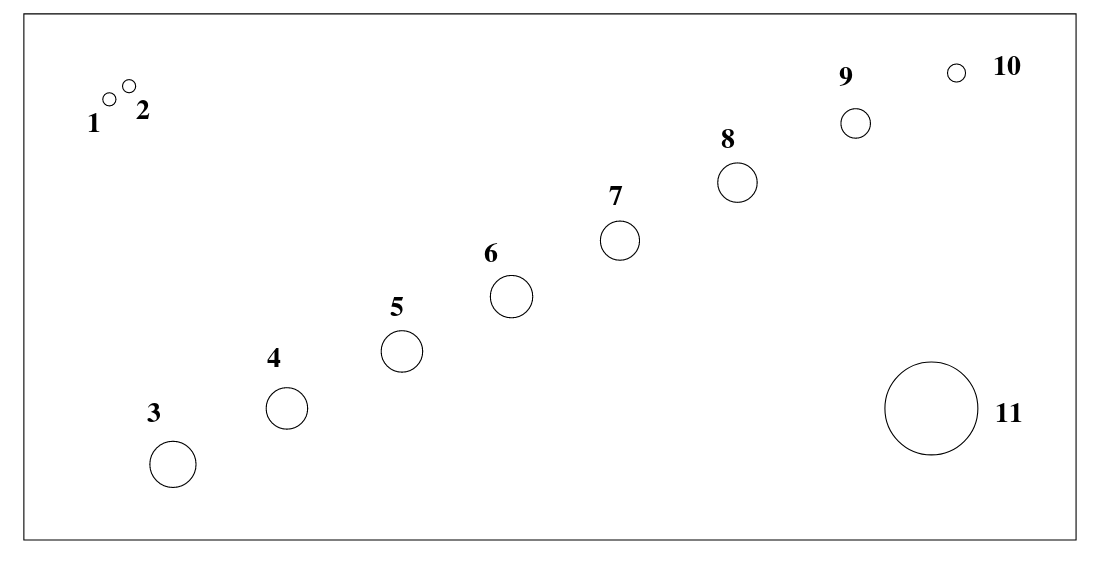
\includegraphics[width=0.8\textwidth]{content/block.png}
    \caption{Struktur des Acrylblocks. \cite{us2}}
    \label{blockloch}
\end{figure}
\noindent
Diese werden zum einen mit der Schieblehre, zum anderen mit der Sonde je von der Unterseite und der Oberseite des Blocks vermessen, um die Durchmesser der Löcher berechnen zu können.
Der Computer wird dabei auf den A-Modus eingestellt.
Die verwendete Sonde misst mit einer Frequenz von \SI{2}{\mega\hertz}.
Es ist besonders zu untersuchen, wie die nahe beieinander gelegenen Löcher 1 und 2 aufgelöst werden und ob Löcher 10 und 11 von beiden Seiten zu messen sind.
Zusätzlich wird an einer Stelle gemessen, an der keine Bohrung ist, um den erhaltenen Wert mit der Gesamthöhe des Blocks zu vergleichen und 
die Laufzeitkorrektur durch die Schutzschicht berücksichtigen zu können.
Anschließend werden die Löcher 1 und 2 mit einer \SI{4}{\mega\hertz}-Sonde untersucht.


Der Computer wird nun auf den B-Modus gestellt und der Block erneut vermessen.
Dafür wird die \SI{2}{\mega\hertz}-Sonde langsam und möglichst gleichmäßig über den Block geführt und aus dem entstehenden Bild die Tiefe der Bohrungen ermittelt.
Auch hier wird einem von oben und einmal von unten gemessen.
\subsection{Vermessung des Herzmodells}
Das sehr stark vereinfachte Herzmodell besteht aus zwei Behältern, zwischen denen eine Membran gespannt ist. 
Diese kann durch eine Handpumpe am unteren Behälter aufgeblasen werden.
Die \SI{2}{\mega\hertz}-Sonde wird so platziert, dass es auf die Membran zeigt und bei voller Auslenkung dieser, sie gerade nicht berührt.
Nun wird so viel Wasser eingefüllt, dass die Sonde zu jedem Zeitpunkt das Wasser berührt.
Der Abstand zu Membran wird im A-Scan Modus einmal im Ausgangszustand und einmal im aufgeblasenen Zustand gemessen.
Anschließend wird manuell ein Herzschlag simuliert und dieser mittels eines TM-Scans aufgenommen.
Aus dem erhaltenen Bild lässt sich die Herzfrequenz und mit der Annahme, dass die Herzmembran annähernd eine Kugelschalge bildet, 
auch der mittlere Herzvolumenstrom berechnen.
